\documentclass[tikz,border=2pt]{standalone}
\usepackage{tikz}
\usetikzlibrary{arrows.meta,positioning}
\begin{document}
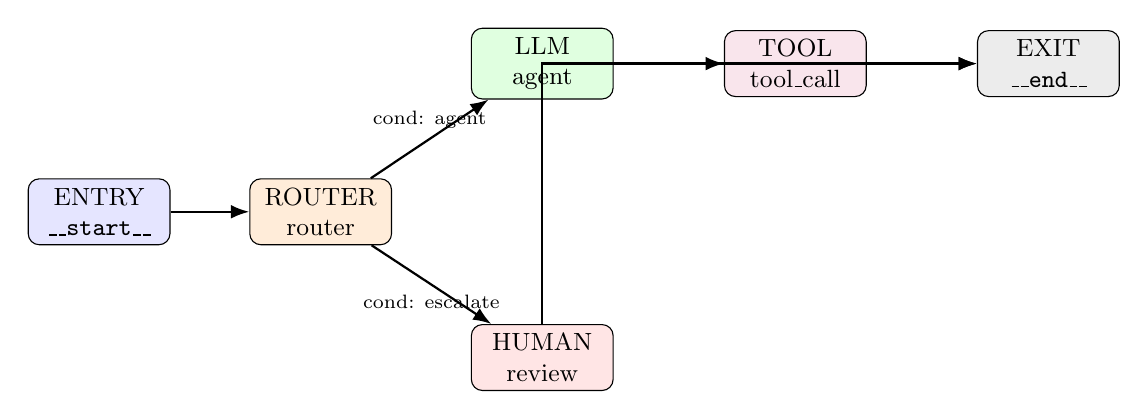
\begin{tikzpicture}[
  node/.style={draw, rounded corners, align=center, minimum width=18mm, minimum height=7mm, font=\small},
  entry/.style={node, fill=blue!10},
  exit/.style={node, fill=gray!15},
  router/.style={node, fill=orange!15},
  llm/.style={node, fill=green!12},
  tool/.style={node, fill=purple!10},
  human/.style={node, fill=red!10},
  arrow/.style={-{Latex}, thick},
]
  \node[entry] (start) {ENTRY\\\texttt{\_\_start\_\_}};
  \node[router, right=10mm of start] (router) {ROUTER\\router};

  \node[llm, above right=10mm and 10mm of router] (agent) {LLM\\agent};
  \node[human, below right=10mm and 10mm of router] (human) {HUMAN\\review};

  \node[tool, right=14mm of agent] (tool) {TOOL\\tool\_call};
  \node[exit, right=14mm of tool] (end) {EXIT\\\texttt{\_\_end\_\_}};

  \draw[arrow] (start) -- (router);
  \draw[arrow] (router) -- node[above, font=\scriptsize]{cond: agent} (agent);
  \draw[arrow] (router) -- node[below, font=\scriptsize]{cond: escalate} (human);
  \draw[arrow] (agent) -- (tool);
  \draw[arrow] (human) |- (end);
  \draw[arrow] (tool) -- (end);
\end{tikzpicture}
\end{document}

